\documentclass{article}
\usepackage{tikz}
\usetikzlibrary{automata,positioning}

\begin{document}

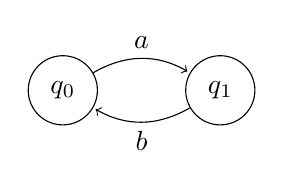
\begin{tikzpicture}[shorten >=1pt,node distance=2cm,on grid,auto]
    \node[state] (q_0) {$q_0$};
    \node[state] (q_1) [right=of q_0] {$q_1$};
    
    \path[->]
        (q_0) edge [bend left] node {$a$} (q_1)
        (q_1) edge [bend left] node {$b$} (q_0);
\end{tikzpicture}

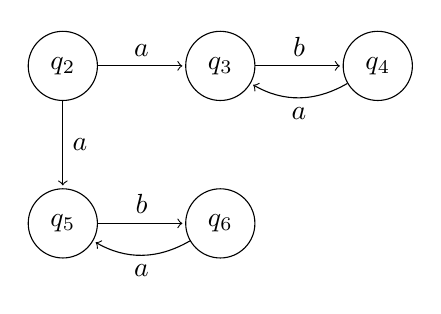
\begin{tikzpicture}[shorten >=1pt,node distance=2cm,on grid,auto]
    \node[state] (q_2) {$q_2$};
    \node[state] (q_3) [right=of q_2] {$q_3$};
    \node[state] (q_4) [right=of q_3] {$q_4$};
    \node[state] (q_5) [below=of q_2] {$q_5$};
    \node[state] (q_6) [right=of q_5] {$q_6$};
    
    \path[->]
        (q_2) edge node {$a$} (q_3)
        (q_3) edge node {$b$} (q_4)
        (q_4) edge [bend left] node {$a$} (q_3)
        (q_2) edge node {$a$} (q_5)
        (q_5) edge node {$b$} (q_6)
        (q_6) edge [bend left] node {$a$} (q_5);
\end{tikzpicture}

\end{document}